%\begin{center}
%	\textbf{{\Huge ĐỀ 002}}
%\end{center}
\subsubsection*{Phần I. Thí sinh trả lời từ câu 1 đến câu 12, mỗi câu hỏi chọn một phương án.}
\setcounter{bt}{0}
\begin{baitap}
	Cho hàm số $y = \dfrac{x + 1}{x - 3}$. Trong các mệnh đề sau, mệnh đề nào \textbf{sai}?
	\begin{enumerate}[\quad \bf A.]
		\item Hàm số nghịch biến trên từng khoảng xác định của nó.
		\item Hàm số nghịch biến trên tập xác định của nó.
		\item Hàm số nghịch biến trên khoảng $(3; +\infty)$.
		\item Hàm số nghịch biến trên khoảng $(-\infty; 3)$.
	\end{enumerate}
\end{baitap}

\begin{baitap}
	Cho hàm số $y = \frac{1}{3}x^3 - \frac{1}{2}x^2 - 12x - 1$. Mệnh đề nào sau đây đúng?
	\begin{multicols}{2}
		\begin{enumerate}[\quad \bf A.]
		\item Hàm số nghịch biến trên khoảng $(-3; +\infty)$.
		\item Hàm số đồng biến trên khoảng $(-\infty; 4)$.
		\item Hàm số đồng biến trên khoảng $(-3; 4)$.
		\item Hàm số đồng biến trên khoảng $(4; +\infty)$.
	\end{enumerate}
	\end{multicols}
\end{baitap}

\begin{baitap}
	Hàm số nào không đồng biến trên $(-\infty; +\infty)$?
	\begin{multicols}{4}
		\begin{enumerate}[\quad \bf A.]
			\item $y = x^5 + x^3 - 1$.
			\item $y = x^3 + 2$.
			\item $y = \frac{x - 1}{x + 2}$.
			\item $y = x + 1$.
		\end{enumerate}
	\end{multicols}
\end{baitap}

\begin{baitap}
	Cho hàm số $y = x - 2\sqrt{x}$. Mệnh đề nào đúng?
	\begin{multicols}{2}
		\begin{enumerate}[\quad \bf A.]
		\item Hàm số nghịch biến trên khoảng $(1; +\infty)$.
		\item Hàm số đồng biến trên khoảng $(2; +\infty)$.
		\item Hàm số đồng biến trên khoảng $(0; +\infty)$.
		\item Hàm số nghịch biến trên khoảng $(-\infty; 1)$.
	\end{enumerate}
	\end{multicols}
\end{baitap}
\begin{baitap}
	Hàm số $y = x^4 - 2x^2 + 1$ đồng biến trên khoảng nào dưới đây?
	\begin{multicols}{4}
		\begin{enumerate}[\quad \bf A.]
			\item $(-1;0)$.
			\item $(-1;+\infty)$.
			\item $(-3;8)$.
			\item $(-\infty;-1)$.
		\end{enumerate}
	\end{multicols}
\end{baitap}

\begin{baitap}
	Cho hàm số $y = f(x)$ xác định và liên tục trên $\mathbb{R}$, có bảng biến thiên như hình sau. Tìm khẳng định đúng.
	\begin{center}
		
\begin{tikzpicture}[scale=.8]
		\tkzTabInit[lgt=1.2, espcl=3]{$x$ /1, $y'$ /1, $y$ /2}{$-\infty$, $2$, $+\infty$}
		\tkzTabLine{, -, 0, +, }
		\tkzTabVar{+/ $+\infty$, -/ $0$, +/ $+\infty$}
	\end{tikzpicture}
	\end{center}
%	\begin{multicols}{2}
		\begin{enumerate}[\quad \bf A.]
		\item Hàm số có 2 cực trị.
		\item Hàm số có giá trị cực đại bằng 2.
		\item Hàm số có giá trị cực tiểu bằng 0.
		\item Hàm số đạt cực đại tại $x = 0$.
	\end{enumerate}
%	\end{multicols}
\end{baitap}


\begin{baitap}
	Cho hàm số $y = f(x)$ có bảng biến thiên như sau. Mệnh đề nào dưới đây là \textbf{sai}?
	
	\begin{center}
		
\begin{tikzpicture}[scale=.8]
		\tkzTabInit[lgt=1.2, espcl=3]{$x$ /1, $y'$ /1, $y$ /2}{$-\infty$, $0$, $2$, $+\infty$}
		\tkzTabLine{, +, 0, -, 0, +, }
		\tkzTabVar{-/ $-\infty$, +/ $3$, -/ $0$, +/ $+\infty$}
	\end{tikzpicture}
	\end{center}	
	\begin{multicols}{2}
		\begin{enumerate}[\quad \bf A.]
		\item Hàm số \textbf{không} đạt cực tiểu tại điểm $x = 2$.
		\item Hàm số đạt cực đại tại điểm $x = 0$.
		\item Giá trị cực đại của hàm số là $y = 3$.
		\item Giá trị cực tiểu của hàm số là $y = 0$.
	\end{enumerate}
	\end{multicols}
\end{baitap}

\begin{baitap}
	Cho hàm số $y = f(x)$ có bảng biến thiên như sau. 	Tìm giá trị cực đại $y_{\text{CĐ}}$ và giá trị cực tiểu $y_{\text{CT}}$ của hàm số.
	\begin{center}
		
\begin{tikzpicture}[scale=.8]
		\tkzTabInit[lgt=1.2, espcl=3]{$x$ /1, $y'$ /1, $y$ /2}{$-\infty$, $0$, $2$, $+\infty$}
		\tkzTabLine{, +, 0, -, 0, +, }
		\tkzTabVar{-/ $-\infty$, +/ $3$, -/ $0$, +/ $+\infty$}
	\end{tikzpicture}
	\end{center}

	\begin{multicols}{2}
		\begin{enumerate}[\quad \bf A.]
		\item $y_{\text{CĐ}} = 3$ và $y_{\text{CT}} = 2$.
		\item $y_{\text{CĐ}} = 2$ và $y_{\text{CT}} = 0$.
		\item $y_{\text{CĐ}} = 3$ và $y_{\text{CT}} = 3$.
		\item $y_{\text{CĐ}} = 3$ và $y_{\text{CT}} = 0$.
	\end{enumerate}
	\end{multicols}
\end{baitap}
\begin{baitap}
	Cho hàm số $y = -\dfrac{1}{4}x^4 + \dfrac{1}{2}x^2 - 3$. Khẳng định nào sau đây là khẳng định đúng?
	\begin{multicols}{2}
		\begin{enumerate}[\quad \bf A.]
			\item Hàm số đạt cực tiểu tại $x = -3$.
			\item Hàm số đạt cực tiểu tại $x = 0$.
			\item Hàm số đạt cực đại tại $x = 0$.
			\item Hàm số đạt cực tiểu tại $x = -1$.
		\end{enumerate}
	\end{multicols}
\end{baitap}
\begin{baitap}
%	\textbf{Câu 8.}	
	Cho hàm số có đồ thị như hình bên. Khẳng định nào \textbf{sai}?
	
	\begin{minipage}{0.65\textwidth}
		\begin{enumerate}[\quad \bf A.]
			\item Hàm số có một cực tiểu tại $x = \dfrac{3}{4}$ và đạt cực đại tại $x = 0$.
			\item Giá trị cực đại $y = -1$ và giá trị cực tiểu $y = -\dfrac{113}{32}$.
			\item Hàm số có một cực tiểu tại $x = -\dfrac{3}{4}$.
			\item Hàm số có một cực đại tại $x = -\dfrac{3}{4}$.
		\end{enumerate}
	\end{minipage}
\begin{minipage}{0.3\textwidth}
		% Graph of a biquadratic function y = ax^4 + bx^2 + c with 3 extrema
		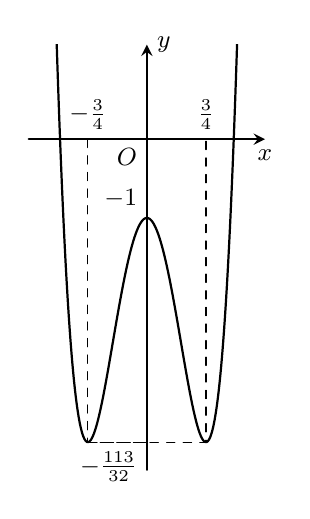
\begin{tikzpicture}[line cap=round, line join=round, >=stealth, scale=1, font=\small]
			% Define window bounds
			\def\xmin{-1.5} \def\xmax{1.5}
			\def\ymin{-4.2} \def\ymax{1.2}
			
			% Macros for key values
			\pgfmathsetmacro{\xA}{-0.75} % -3/4
			\pgfmathsetmacro{\xB}{0.75}  %  3/4
			\pgfmathsetmacro{\yMin}{-3.85} % -113/32 = -3.53125
			\pgfmathsetmacro{\yMax}{-1}
			
			% Curve fitting: y = a*x^4 + b*x^2 + c
			% Local max at (0, -1) => c = -1
			% Local min at (+-3/4, -113/32) => f'(3/4) = 0 and f(3/4) = -113/32
			% Yields: a = 9, b = -10.125 (-81/8), c = -1
			
			\begin{scope}
				\clip (\xmin,\ymin) rectangle (\xmax,\ymax);
				
				% Graph of y = 9*x^4 - (81/8)*x^2 - 1
				\draw[black, thick, smooth, samples=200, domain=\xmin:\xmax]
				plot(\x, {9*(\x)^4 - (81/8)*(\x)^2 - 1});
			\end{scope}
			
			% Dashed lines connecting extrema to axes
			\draw[dashed, thin] (\xA,0) -- (\xA,\yMin) -- (\xB,\yMin) -- (\xB,0);
			\draw[dashed, thin] (0,\yMin) -- (\xA,\yMin);
			
			% Draw Axes
			\draw[->, thick] (\xmin,0) -- (\xmax,0) node[below]{$x$};
			\draw[->, thick] (0,\ymin) -- (0,\ymax) node[right]{$y$};
			
			% Labels and Values
			\node[below left] at (0,0) {$O$};
			\node[above left] at (0,-1) {$-1$};
			\node[above] at (\xA,0) {$-\frac{3}{4}$};
			\node[above] at (\xB,0) {$\frac{3}{4}$};
			\node[below left] at (0,\yMin) {$-\frac{113}{32}$};
		\end{tikzpicture}	
\end{minipage}
\end{baitap}
\begin{baitap}
	Tìm tất cả các giá trị của tham số $m$ để hàm số $y = x^3 + mx^2 + (1 - 2m)x + m - 3$ đồng biến trên khoảng $(-3;0)$.
	\begin{multicols}{4}
		\begin{enumerate}[\quad \bf A.]
			\item $m \ge 2\sqrt{3} + 3$.
			\item $m \le 2\sqrt{3} - 3$.
			\item $m \ge 6 - \sqrt{42}$.
			\item $m \le 6 + \sqrt{42}$.
		\end{enumerate}
	\end{multicols}
\end{baitap}

\begin{baitap}
	Tìm tất cả các giá trị của tham số $m$ sao cho hàm số $y = -x^3 - 3mx^2 + 4m - 1$ đồng biến trên khoảng $(0;4)$.
	\begin{multicols}{4}
		\begin{enumerate}[\quad \bf A.]
			\item $-2 \le m < 0$.
			\item $m \le -4$.
			\item $m \le -2$.
			\item $m > 0$.
		\end{enumerate}
	\end{multicols}
\end{baitap}

%\begin{baitap}
%	Tìm tất cả các giá trị của tham số $m$ để hàm số $y = -x^3 + 3x^2 + 3mx - 1$ nghịch biến trên khoảng $(0;+\infty)$.
%	\begin{multicols}{4}
%		\begin{enumerate}[\quad \bf A.]
%			\item $m > -1$.
%			\item $m \ge -1$.
%			\item $m \le -1$.
%			\item $m < -1$.
%		\end{enumerate}
%	\end{multicols}
%\end{baitap}


\subsubsection*{Phần II. Thí sinh trả lời từ câu 1 đến câu 4, trong ý a), b), c), d) ở mỗi câu câu, thí sinh chọn ĐÚNG hoặc SAI}.
\setcounter{bt}{0}
\begin{baitap} %Câu 1 BGD Lần 2 2026
	Cho hàm số $y=f(x)=x^3-6x^2+9x+2$.
	\begin{enumerate}[\quad \bf a)]
		\item Đạo hàm của hàm số đã cho là $f'(x)=3x^2-12x+9$.
		\item Phương trình $f'(x)=0$ có tập nghiệm là $S=\{1;3\}$.
%		\item Hàm số đã cho đạt giá trị lớn nhất trên đoạn $[2;4]$ tại $x=2$.
	\item Hàm số đã cho đồng biến trên đoạn $ [4;5] $.
		\item Gọi $x_1, x_2$ là hai điểm cực trị của hàm số $y=f(x)$. Khi đó, phương trình đường thẳng đi qua hai điểm $M_1(x_1; f(x_1))$ và $M_2(x_2; f(x_2))$ là $y=-2x+1$.
	\end{enumerate}
\end{baitap}
\begin{baitap}
	Cho hàm số $y=f(x)$ xác định trên $\mathbb{R}$ và có bảng xét dấu của đạo hàm như hình vẽ.
	\begin{center}
		%!<\usepackage{tkz-tab}>
		
		
\begin{tikzpicture}[scale=.8]
			% Sign table for derivative f'(x) based on provided image
			\tkzTabInit[lgt=1.5, espcl=3]
			{$x$ / 1, $f'(x)$ / 1}
			{$-\infty$, $-1$, $1$, $+\infty$}
			
			\tkzTabLine{, +, z, -, z, +, }
		\end{tikzpicture}
	\end{center}
%	\begin{multicols}{2}
		\begin{enumerate}[\quad \bf a)]
		\item Hàm số có $2$ cực trị.
		\item Hàm số nghịch biến trên khoảng $(-1; 1)$.
		\item Hàm số đồng biến trên khoảng $(1; +\infty)$.
		\item Hàm số $f(1-x)$ đồng biến trên khoảng $(-1; 1)$.
	\end{enumerate}
%	\end{multicols}
\end{baitap}


\begin{baitap}
	Cho hàm số $y = \dfrac{x^2 + 2x + 2}{x + 1}$ có đồ thị (C). Gọi $A, B$ lần lượt là điểm cực tiểu và điểm cực đại của (C).
	\begin{enumerate}[\quad \bf a)]
		\item Tập xác định của hàm số là $\mathbb{R}$.
		\item Hàm số nghịch biến trên khoảng $(-2; 0)$.
		\item Tọa độ điểm $A(-2; -2)$, $B(0; 2)$.
		\item Khoảng cách giữa hai điểm cực trị là $AB = 2\sqrt{5}$.
	\end{enumerate}
\end{baitap}

\begin{baitap}
	Một chất điểm chuyển động dọc theo trục $Ox$ có tọa độ tại thời điểm $t$ xác định bởi $x(t) = t^3 - 6t^2 + 9t$ với $t \ge 0$. Khi đó $v(t)=x'(t),a(t)=v'(t)$ là vận tốc và gia tốc của chất điểm tại thời điểm $t$.
	\begin{enumerate}[\quad \bf a)]
		\item Phương trình hàm vận tốc là $v(t) = 3t^2 - 6t + 9$.
		\item Phương trình hàm gia tốc là $a(t) = 6t - 12$.
		\item Vận tốc của chất điểm tăng khi $t \in (0; 1)$ hoặc $t \in (3; +\infty)$.
		\item Vận tốc của chất điểm giảm khi $t \in (1; 3)$.
	\end{enumerate}
\end{baitap}

%\begin{baitap}
%	Đạo hàm $f'(x)$ của hàm số $y=f(x)$ có đồ thị như hình bên dưới.
%	\begin{center}
%		% Graph of y = f'(x) cubic curve passing through (-1,0), (2,0), (4,0) on [-2, 5]
%		\begin{tikzpicture}[line cap=round, line join=round, >=stealth, scale=0.8]
%			% Define plotting window
%			\def\xmin{-2.8} \def\xmax{5.8}
%			\def\ymin{-2.5} \def\ymax{2.5}
%			
%			% Function: f'(x) = k*(x+1)*(x-2)*(x-4) = k*(x^3 - 5x^2 + 2x + 8)
%			% Using k = 0.12 for reasonable vertical scale
%			
%			\begin{scope}
%				\clip (\xmin,\ymin-1) rectangle (\xmax,\ymax);
%				
%				% Graph of y = f'(x) on [-2, 5]
%				\draw[black, smooth, samples=200, domain=-2:5]
%				plot(\x, {0.12*((\x)^3 - 5*(\x)^2 + 2*(\x) + 8)});
%			\end{scope}
%			
%			% Dashed vertical lines at boundaries x = -2 and x = 5
%			\draw[dashed, thin] (-2,0) -- (-2, {0.12*((-2)^3 - 5*(-2)^2 + 2*(-2) + 8)});
%			\draw[dashed, thin] (5,0) -- (5, {0.12*((5)^3 - 5*(5)^2 + 2*(5) + 8)});
%			
%			% Coordinate Axes
%			\draw[->, thick] (\xmin,0) -- (\xmax,0) node[below]{$x$};
%			\draw[->, thick] (0,\ymin) -- (0,\ymax) node[left]{$y$};
%			
%			% Key x-intercept points (roots at -1, 2, 4)
%			\fill (-1,0) circle (1.5pt);
%			\fill (2,0) circle (1.5pt);
%			\fill (4,0) circle (1.5pt);
%			
%			% Axis & point labels
%			\node[below right] at (0,0) {$O$};
%			\node[below left] at (-2,0) {$-2$};
%			\node[below right] at (-1,0) {$-1$};
%			\node[below left] at (2,0) {$2$};
%			\node[below right] at (4,0) {$4$};
%			\node[below] at (5,0) {$5$};
%			
%			% Function label y = f'(x)
%			\node[above left] at (4.8, 1.3) {$y=f'(x)$};
%		\end{tikzpicture}
%	\end{center}
%	
%	\begin{multicols}{2}
%		\begin{enumerate}[\quad \bf a)]
%		\item Hàm số đạt cực tiểu tại $x=-1$.
%		\item Hàm số đồng biến trên $(-1; 2)$ và $(4; 5)$.
%		\item Hàm số nghịch biến trên $(2; 4)$.
%		\item Hàm số $f(x+2)$ đạt cực đại tại $x=0$.
%	\end{enumerate}
%	\end{multicols}
%\end{baitap}


%\begin{baitap}
%	Cho hàm số $y=f(x)$ xác định trên $\mathbb{R}$ và có đồ thị của hàm số $y=f'(x)$ là đường cong ở hình vẽ dưới.
%	\begin{center}
%		% Cubic function y = f'(x) with local max at (0,2) and local min at (2,-2)
%		\begin{tikzpicture}[line cap=round, line join=round, >=stealth, scale=0.85]
%			% Define window bounds
%			\def\xmin{-2.2} \def\xmax{3.2}
%			\def\ymin{-2.8} \def\ymax{2.8}
%			
%			% Scope to clip the curve within window bounds
%			\begin{scope}
%				\clip (\xmin,\ymin) rectangle (\xmax,\ymax);
%				
%				% Graph of f'(x) = x^3 - 3x^2 + 2
%				\draw[black, thick, smooth, samples=200, domain=\xmin:\xmax]
%				plot(\x, {(\x)^3 - 3*(\x)^2 + 2});
%			\end{scope}
%			
%			% Dashed lines connecting critical point (2,-2) to coordinate axes
%			\draw[dashed, thin] (2,0) -- (2,-2) -- (0,-2);
%			
%			% Draw Coordinate Axes
%			\draw[->, thick] (\xmin,0) -- (\xmax,0) node[below]{$x$};
%			\draw[->, thick] (0,\ymin) -- (0,\ymax) node[left]{$y$};
%			
%			% Labels and Key Values
%			\node[below left] at (0,0) {$O$};
%			\node[left] at (0,2) {$2$};
%			\node[left] at (0,-2) {$-2$};
%			\node[above] at (2,0) {$2$};
%			
%			% Curve label
%			\node[above left] at (2.5, 2.0) {$y = f'(x)$};
%		\end{tikzpicture}
%	\end{center}
%	\begin{enumerate}[\quad \bf a)]
%		\item Hàm số $f(x)$ đạt cực đại tại $x=0$.
%		\item Hàm số $f(x)$ nghịch biến trong khoảng $(0;2)$.
%		\item Hàm số $f(x)$ có 2 khoảng đồng biến và 2 khoảng nghịch biến.
%		\item Hàm số $f(x)$ có 3 điểm cực trị.
%	\end{enumerate}
%\end{baitap}

%\begin{baitap}
%	\textbf{Câu 4.} Cho hàm số $y=f(x)$ liên tục trên đoạn $\left[0; \frac{16}{5}\right]$ thoả mãn $f'\left(\frac{1}{3}\right) = f'(1) = f'\left(\frac{5}{2}\right) = 0$ và có đồ thị là đường cong như hình dưới.
%	\begin{center}
%		\begin{tikzpicture}[line cap=round, line join=round, >=stealth, scale=1.2]
%			% Define plotting domain and bounding box
%			\def\xmin{-0.8} \def\xmax{3.8}
%			\def\ymin{-2.8} \def\ymax{3.6}
%			
%			% Define exact values/coordinates
%			\pgfmathsetmacro{\xA}{1/3}
%			\pgfmathsetmacro{\xB}{1}
%			\pgfmathsetmacro{\xC}{2.5}     % 5/2
%			\pgfmathsetmacro{\xD}{3.2}     % 16/5
%			
%			% Scope to clip the curve safely within bounds
%			\begin{scope}
%				\clip (\xmin,\ymin) rectangle (\xmax,\ymax);
%				
%				% Polynomial fitting points:
%				% f(0) = 0, f(1/3) = -1/3 (local min), f(1) = 0 (local max),
%				% f(5/2) = -2 (local min), f(16/5) = 3
%				\draw[black, thick, smooth, samples=200, domain=0:\xD]
%				plot(\x, {1.8687*(\x)^4 - 10.465*(\x)^3 + 17.58*(\x)^2 - 8.9837*(\x)});
%			\end{scope}
%			
%			% Dashed projection lines
%			\draw[dashed, thin] (0,3) -- (\xD,3) -- (\xD,0);
%			\draw[dashed, thin] (0,-2) -- (\xC,-2) -- (\xC,0);
%			
%			% Draw Coordinate Axes
%			\draw[->, thick] (\xmin,0) -- (\xmax,0) node[below]{$x$};
%			\draw[->, thick] (0,\ymin) -- (0,\ymax) node[right]{$y$};
%			
%			% Labels and Key Values on Axes
%			\node[above left] at (0,0) {$O$};
%			
%			% X-axis ticks & labels
%			\draw (\xA,2pt) -- (\xA,-2pt) node[above=2pt, font=\small] {$\frac{1}{3}$};
%			\draw (\xB,2pt) -- (\xB,-2pt) node[above=1pt, font=\small] {$1$};
%			\draw (\xC,2pt) -- (\xC,-2pt) node[above=1pt, font=\small] {$\frac{5}{2}$};
%			\draw (\xD,2pt) -- (\xD,-2pt) node[below=1pt, font=\small] {$\frac{16}{5}$};
%			
%			% Y-axis ticks & labels
%			\node[left] at (0,3) {$3$};
%			\node[left] at (0,-1/3) {$-\frac{1}{3}$};
%			\node[left] at (0,-2) {$-2$};
%			
%		\end{tikzpicture}
%	\end{center}
%	\begin{enumerate}[\quad \bf a)]
%		\item $x=1$ là điểm cực đại của hàm số.
%		\item $x=\dfrac{1}{3}$, $x=\dfrac{5}{2}$ là điểm cực tiểu của hàm số.
%		\item Hàm số đã cho nghịch biến trên $\left(\dfrac{1}{3}; 1\right)$ và $\left(\dfrac{5}{2}; +\infty\right)$.
%		\item Giá trị lớn nhất của hàm số là $3$.
%	\end{enumerate}
%\end{baitap}


\subsubsection*{Phần III. Thí sinh trả lời từ câu 1 đến câu 6 (không làm tròn các phép tính trung gian trong các câu từ 1 đến câu 6).}
\setcounter{bt}{0}
\begin{baitap}
	Cho hàm số $y = f(x) = \dfrac{2x^2 + 12x + 8}{x + 6}$ có giá trị cực tiểu bằng $y_1$ và giá trị cực đại bằng $y_2$. Tính $P = -y_1 + 2y_2$, (kết quả làm tròn đến hàng phần mười).
\end{baitap}
\begin{baitap}
	Sau khi một hóa chất bị tràn xuống hồ, nồng độ của hóa chất đó trong nước $C$ (đơn vị: $\text{ppm}$) đo được sau $t$ giờ (kể từ lúc bắt đầu sự cố) tuân theo mô hình:
	\[
	C(t) = -t^3 + 12t^2 + 60t,\quad (0 \le t \le 15)
	\]
	Sau bao nhiêu giờ kể từ lúc sự cố xảy ra thì nồng độ hóa chất trong hồ đạt mức cao nhất? Mức nồng độ cao nhất đó là bao nhiêu $\text{ppm}$?
\end{baitap}

\begin{baitap}
	Hằng ngày mực nước của hồ thủy điện ở miền Trung lên và xuống theo lượng nước mưa, và các suối nước đổ về hồ. Từ  $\SI{8}{h}$ sáng, độ sâu của mực nước trong hồ (tính bằng mét) lên xuống theo thời gian $t$ (giờ) cho bởi công thức $h(t) = 24t + 5t^2 - \dfrac{t^3}{3}$. Biết rằng phải thông báo cho các hộ dân phải di dời trước khi xả nước theo quy định trước $5$ giờ. Hỏi cần thông báo cho hộ dân di dời lúc mấy giờ trong ngày (tính theo $24$ giờ)? Biết rằng mực nước trong hồ phải lên cao nhất mới xả nước.
\end{baitap}
\begin{baitap}
	Cho hàm số $y = \dfrac{mx + 2}{2x + m}$, $m$ là tham số thực. Gọi $S$ là tập hợp tất cả các giá trị nguyên của $m$ để hàm số nghịch biến trên khoảng $(0; 1)$. Tìm số phần tử của $S$.
\end{baitap}

\begin{baitap}
	Tìm giá trị của tham số $m$ để hàm số $f(x) = (m^2 - 3)x - 2m \ln x$ đạt cực tiểu tại điểm $x_0 = 1$.
\end{baitap}

\begin{baitap}
	Gọi $A, B$ là hai điểm cực trị của đồ thị hàm số $y = x^3 - 3x^2 + 4$. Tính diện tích $S$ của tam giác $OAB$ với $O$ là gốc tọa độ.
\end{baitap}

%\begin{baitap}
%	Có bao nhiêu giá trị nguyên của tham số $m$ để hàm số $y = \frac{1}{3}x^3 - (m - 1)x^2 - (m - 3)x + 2024m$ đồng biến trên các khoảng $(-3; -1)$ và $(0; 3)$?
%\end{baitap}